% Requires \usepackage{graphicx}
\begin{figure*}[t]
  \centering
  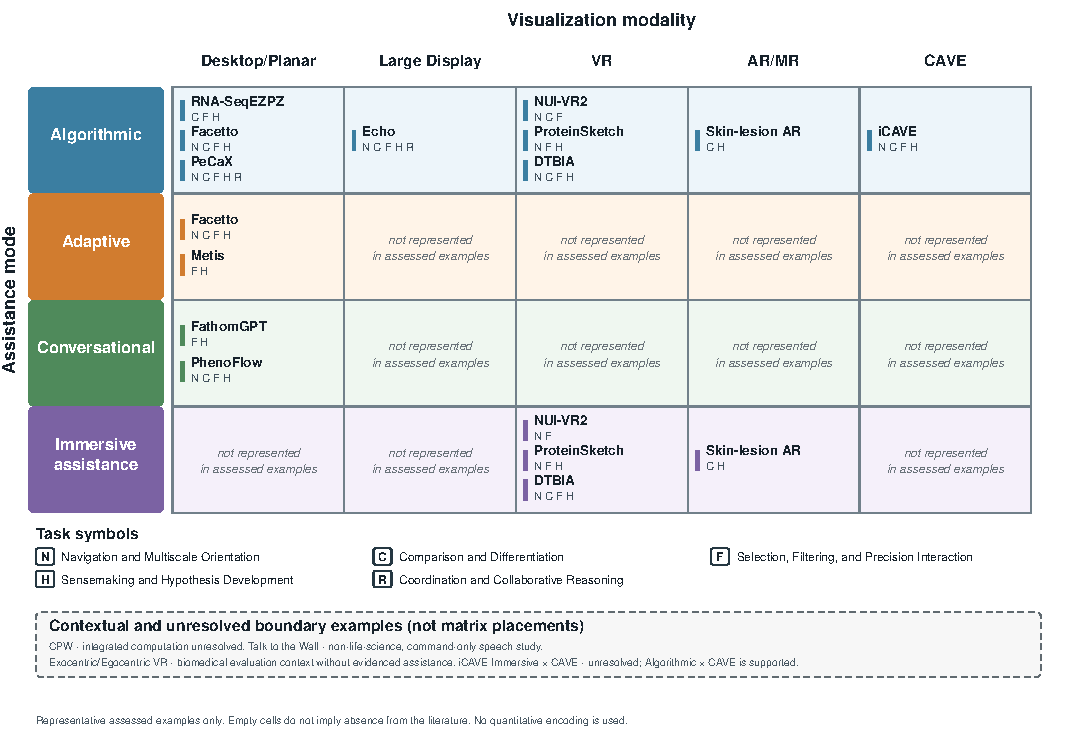
\includegraphics[width=\textwidth]{assistance_visualization_modality_map.pdf}
  \caption{Assistance $\times$ visualization modality in the assessed examples. Rows show the four retained, overlapping assistance modes and columns show the five retained visualization modalities. Task symbols identify supported analytical intents: N, Navigation and Multiscale Orientation; C, Comparison and Differentiation; F, Selection, Filtering, and Precision Interaction; H, Sensemaking and Hypothesis Development; and R, Coordination and Collaborative Reasoning. A system appears in multiple cells only when its full report supports the corresponding assistance-modality mechanism; display type, adjustable parameters, or speech input alone do not create an additional placement. The dashed boundary box identifies contextual or unresolved evidence and is not part of the eligible-example matrix. Empty cells mean that the combination is not represented in these assessed examples, not that no such systems or literature exist. The figure encodes no counts or prevalence.}
  \label{fig:assistance-modality-map}
\end{figure*}
